% Finite-box effect on the halo potential statistics (512^3 production boxes). Figures and table:
% make_boxsize_figures.py; data: data/box512_L200_L500_L1000/.

\subsection{Data}
Three production runs of the pipeline on pawna, $512^3$ particles in boxes of $L = 200$, 500 and 1000\,\Mpch, from
the same seed (\texttt{iSeed} 12345678; same cosmology and output list; \fp{Sahyadri_L<L>N512/default512/r1}). The
statistics are the pipeline stages \texttt{vprof} (volume-weighted stacked potential around host halos,
\fp{halo_potential_profile.py}, grid $1024^3$, at most 20\,000 halos per bin) and \texttt{xcorr} (halo--halo
potential structure function $\langle(\phi_i-\phi_j)^2\rangle$ of $\phi_{R_{\rm vir}}$, pairs within one mass bin,
\fp{halo_potential_xcorr.py}), at $z = 0$, 0.2 and 0.5 (outputs 100, 82, 64), in the three upper mass bins
($M_{\rm vir}=10^{13}$--$5\times10^{13}$, $5\times10^{13}$--$2\times10^{14}$, $2\times10^{14}$--$10^{16}$\,\Msunh).
Errors are jackknife over $3^3$ sub-cubes of halo centres. The same particle number means that the boxes also differ
in mass resolution, by $(1000/200)^3 = 125$ between L200 and L1000: $10^{13}$\,\Msunh{} is 15 particles in L1000, so
its lowest bin used here is incomplete (mean mass $2.5\times10^{13}$ against $2.0\times10^{13}$\,\Msunh{} in the other
boxes). The top bin of L200 holds only 28--76 halos.

\subsection{Shift caused by the periodic box: derivation}
Notation: comoving separation $r$ and wavenumber $k$ in \Mpch{} and $h$\,Mpc$^{-1}$; $\phi$ is the peculiar, physical
potential in \kms{} (the convention of the whole report); Poisson's equation in comoving coordinates is
\begin{equation}
\nabla^2\phi = C\,\delta,\qquad C \equiv 4\pi G\bar\rho a^2 = \tfrac32\,\Omega_m H_0^2\,(1+z),\qquad
H_0 = 100~\mathrm{km\,s^{-1}}\,(h^{-1}\mathrm{Mpc})^{-1}.
\end{equation}
A periodic box imposes two exact conditions that the Universe does not: the density contrast averages to zero over
every box, $\int_V\delta\,d^3x = 0$ (fixed total mass), and $\phi$ repeats with period $L$, so the gradient averages
to zero, $\int_V\nabla\phi\,d^3x = 0$.

\paragraph{Fourier space.} $\phi_{\mathbf k} = -C\,\delta_{\mathbf k}/k^2$. For halos of linear bias $b$, the mean
potential at distance $r$ and the potential correlation function are
\begin{equation}
\langle\phi\rangle(r) = -C\,b\int\!\frac{d^3k}{(2\pi)^3}\,\frac{P(k)}{k^2}\,j_0(kr),\qquad
\xi_{\phi\phi}(r) = C^2\int\!\frac{d^3k}{(2\pi)^3}\,\frac{P(k)}{k^4}\,j_0(kr),
\end{equation}
and the structure function of the halo potentials contains $2[\xi_{\phi\phi}(0)-\xi_{\phi\phi}(r)]$. In the box the
integral becomes a sum over the box modes, $\int d^3k/(2\pi)^3\to L^{-3}\sum_{\mathbf n\neq0}$,
$\mathbf k = 2\pi\mathbf n/L$: modes longer than the box are absent and those near the fundamental
$k_f = 2\pi/L$ are discrete. The shift is (box $-$ infinite), evaluated with both cut at $|k| < 48\,k_f$ (beyond,
sum and integral agree):
\begin{align}
\Delta\langle\phi\rangle(r) &= -C\,b\,\Big[L^{-3}\textstyle\sum_{\mathbf n\neq0} - \int\frac{d^3k}{(2\pi)^3}\Big]
\frac{P(k)}{k^2}\,j_0(kr),\\
\Delta\langle(\phi_i-\phi_j)^2\rangle(r) &= 2C^2\Big[L^{-3}\textstyle\sum_{\mathbf n\neq0} - \int\frac{d^3k}{(2\pi)^3}\Big]
\frac{P(k)}{k^4}\,\big[1-j_0(kr)\big].
\end{align}
The missing modes have $kr\ll1$, so $j_0\simeq1$: the shift of $\langle\phi\rangle$ is nearly independent of $r$
(positive: the box potential is shallower), and with $1-j_0\simeq k^2r^2/6$ the structure-function shift grows as
$r^2$ (negative). $P(k)$ is the CLASS spectrum of the initial conditions at $z = 49$ times the linear growth factor
squared; $b$ is the Tinker et~al.\ (2010) bias at the bin's mean mass (overdensity: Bryan \& Norman virial relative to
the mean density). The structure-function prediction does not depend on the halo bias at this order.

\paragraph{Real space, mean potential.} With the Green's function of Poisson's equation,
$\phi(\mathbf x) = -\frac{C}{4\pi}\int\delta(\mathbf x')/|\mathbf x-\mathbf x'|\,d^3x'$, and the average over halos
turns $\delta$ into the halo--matter correlation $\xi_{hm}$. At the halo centre, by the shell theorem (a shell at $s$
with excess mass $dM$ adds $-G\,dM/s$),
\begin{equation}
\langle\phi\rangle(0) = -C\int_0^\infty\xi_{hm}(s)\,s\,ds .
\end{equation}
The weight $s$ (not $s^2$) makes distant matter count: for the linear $\xi$, 21\% of the integral comes from
$s > 25$\,\Mpch, and the part beyond the zero crossing at 120\,\Mpch{} is negative. In the box the excess mass
around every halo must be paid for by a deficit inside the same box, because the total mass is fixed (integral
constraint; this is what the neutralising background of the Ewald sum does). Model the box as a sphere of the same
volume, $R_L = (3/4\pi)^{1/3}L = 0.62\,L$, with
\begin{equation}
\xi^{\rm box}_{hm}(s) = \xi_{hm}(s) - \bar\xi\ \ (s<R_L),\qquad 0\ \ (s>R_L),\qquad
\bar\xi = \frac{3}{R_L^3}\int_0^{R_L}\xi_{hm}\,s^2\,ds,
\end{equation}
so that $\int\xi^{\rm box}_{hm}\,d^3s = 0$. Then
\begin{equation}
\Delta\langle\phi\rangle = C\,b\left[\bar\xi\,\frac{R_L^2}{2} + \int_{R_L}^\infty\xi(s)\,s\,ds\right].
\end{equation}
The first term is the uniform deficit: tiny in density ($\bar\xi = 0.0036$ for L200 at $z = 0$, $b = 1$) but spread
over the whole box, so its potential grows as $L^2\bar\xi$. The second is the matter that is not there beyond the box;
it is mostly past the zero crossing, negative, and cancels about a quarter of the first ($b = 1$, $z = 0$, in
$10^5$\,\kms: L200 $1.29-0.34 = 0.95$, L500 $0.28-0.09 = 0.19$, L1000 $0.07-0.02 = 0.05$, against 1.07, 0.26, 0.075
from the mode sum). The real-space estimate gives 70--90\% of the mode sum; the rest is the cube and its periodic
images, which the sphere ignores. The shift therefore comes mostly from mass conservation inside the box (the halos'
surroundings are forced to be slightly emptier than in the Universe), not from the absence of distant matter as such.

\paragraph{Real space, structure function.} For two halos at separation $\mathbf r$ the part of the potential that
varies slowly over $r$ gives $\phi_i-\phi_j\simeq-\mathbf g\cdot\mathbf r$, $\mathbf g = -\nabla\phi$. Average the
acceleration over a region $V$: by Newton's third law the internal forces cancel, so $\bar{\mathbf g}_V$ is the pull
of all matter outside $V$. In a periodic box there is no outside (only copies of the box), and indeed
$\int_V\nabla\phi = 0$: the coherent pull on the box as a whole, and the bulk flow it drives, are exactly zero. The
missing part of the structure function is therefore
\begin{equation}
\Delta\langle(\phi_i-\phi_j)^2\rangle \simeq -\frac{\langle\bar g_V^2\rangle\,r^2}{3},\qquad
\langle\bar g_V^2\rangle = C^2\int\frac{d^3k}{(2\pi)^3}\,\frac{P(k)}{k^2}\,W^2(kR_L),
\end{equation}
the variance of the mean acceleration of a sphere of the box volume in an infinite universe ($W$: top-hat window;
the integral is only the convenient way to evaluate this real-space variance). In velocity, $v = f\,aH\,\bar g/C$:
the box removes a bulk flow of 3D rms 195, 97 and 53\,km\,s$^{-1}$ for L200, L500 and L1000 at $z = 0$
(Table~\ref{tab:boxsize}). This captures 60\% of the mode-sum shift: the cube also lacks gradients that vary within
the box on scales $\gtrsim L/2$, not only the uniform one. A second, exact consequence of periodicity needs no model:
$\phi(\mathbf x+L\hat{\mathbf e}) = \phi(\mathbf x)$, so along an axis the structure function returns to zero at
$r = L$ and is symmetric about $L/2$; at 40\,\Mpch{} L200 is already at $0.2\,L$.

\subsection{Results}
\begin{figure}[H]
\centering
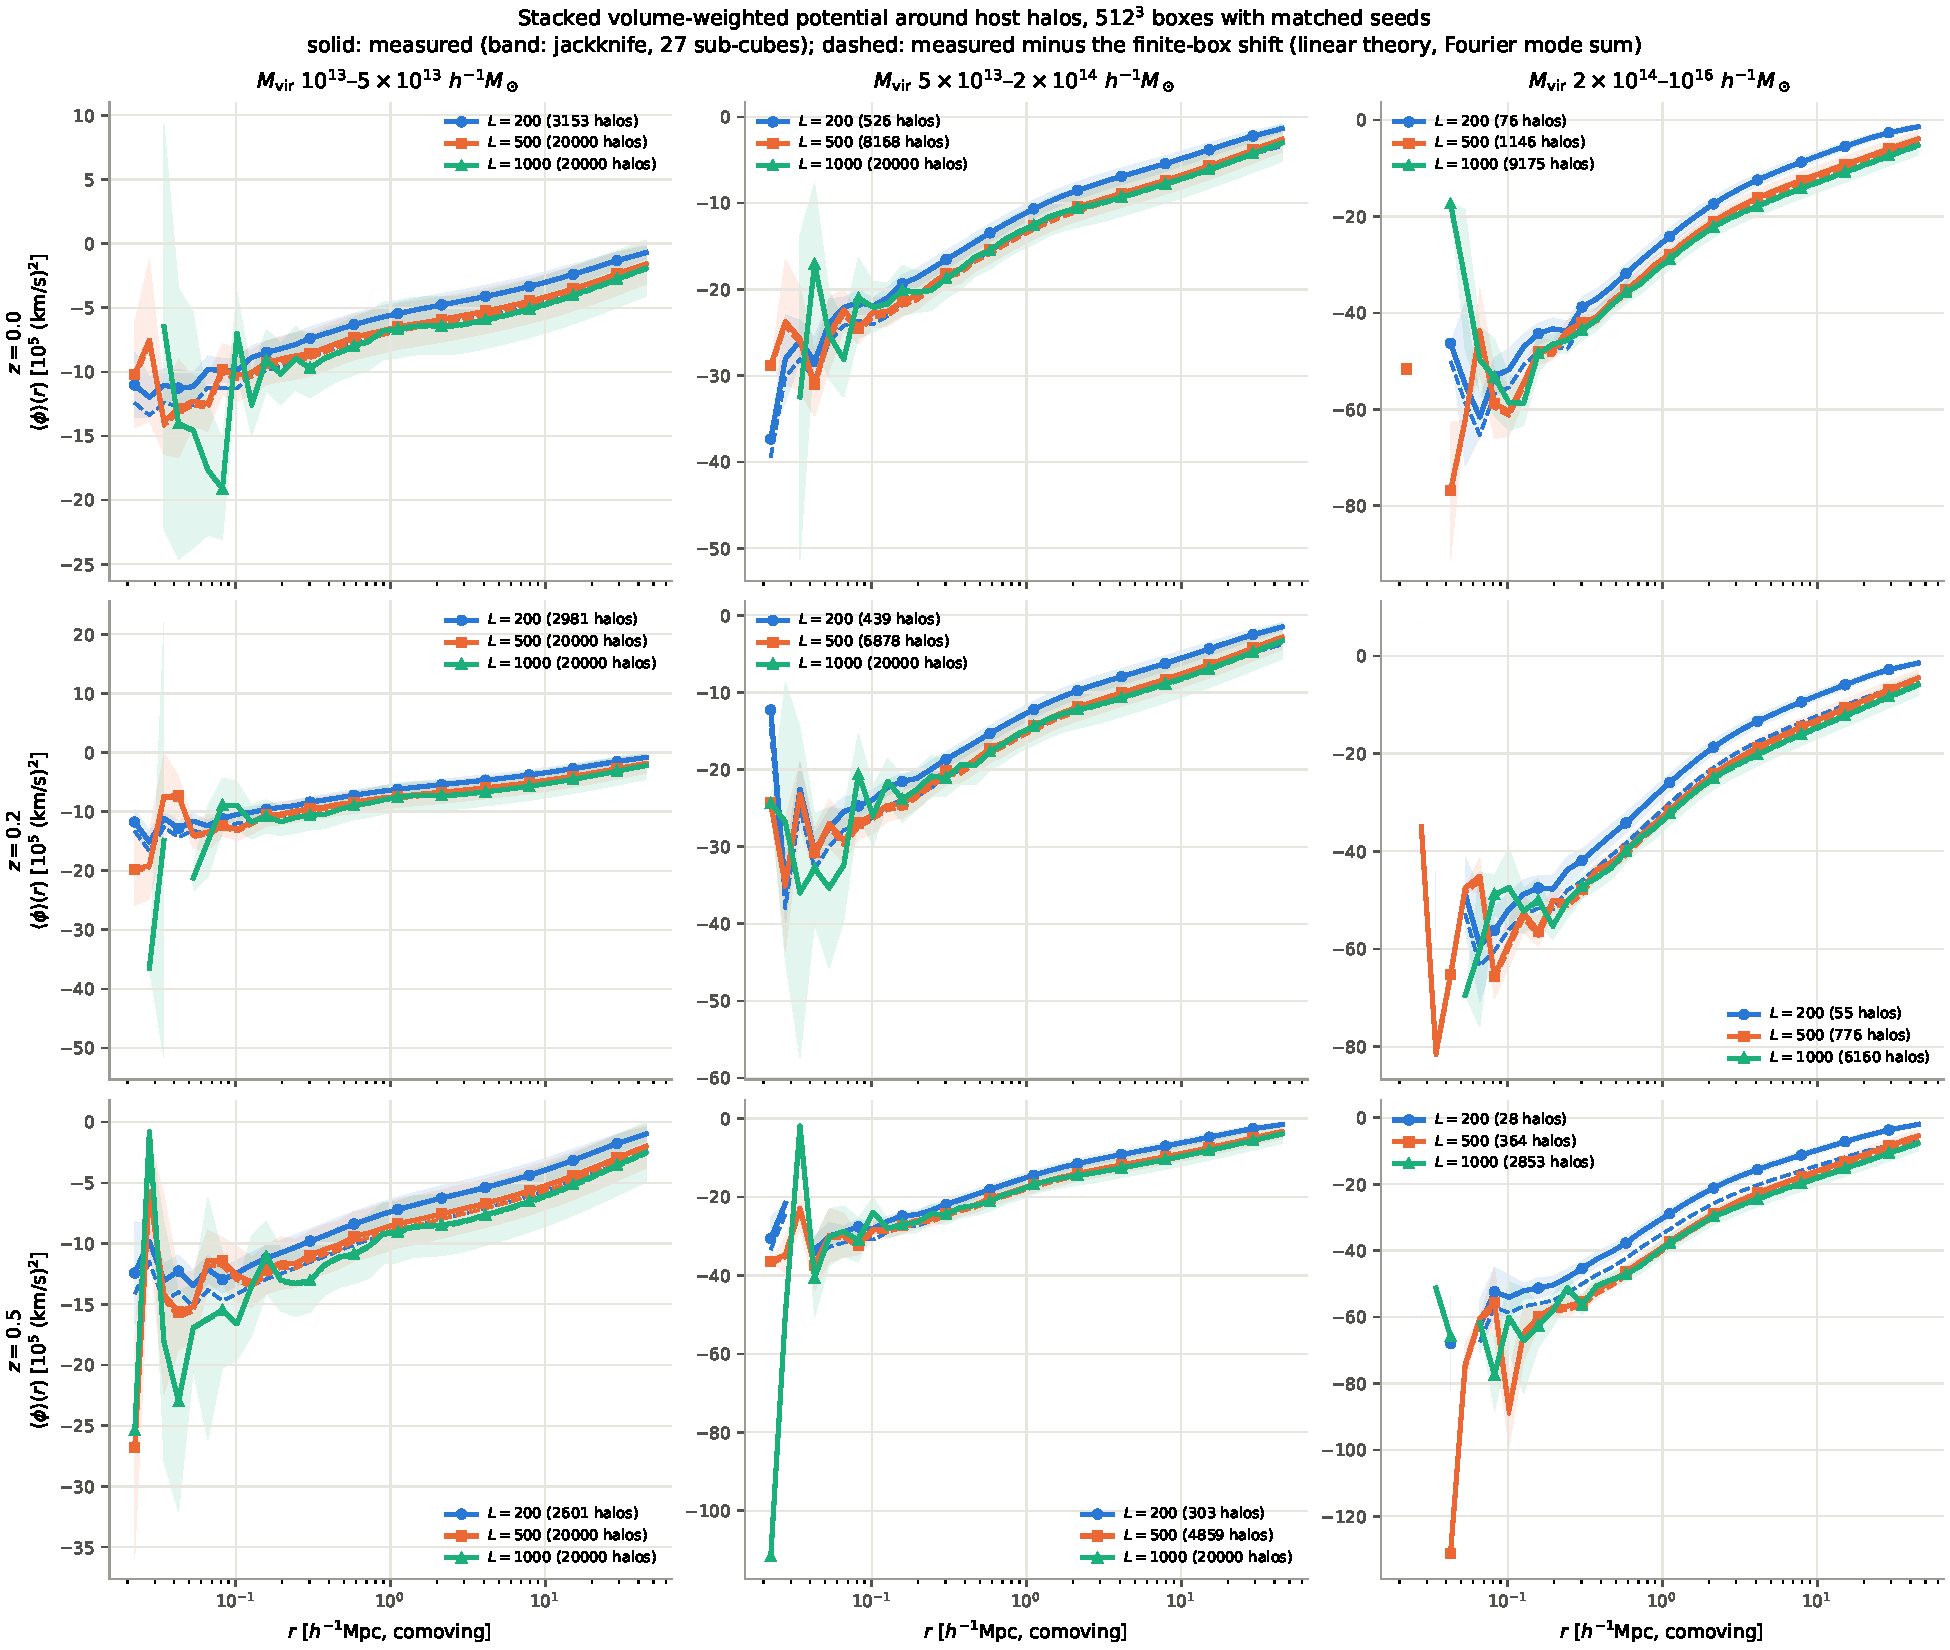
\includegraphics[width=\textwidth]{figs/boxsize_vprof.pdf}
\caption{Stacked volume-weighted potential around host halos in the three boxes (rows: $z$; columns: mass bins).
Solid: measured, band: jackknife error. Dashed: measured minus the predicted shift (mode sum), an estimate of the
infinite-volume profile.}
\label{fig:boxsize_vprof}
\end{figure}

\begin{figure}[H]
\centering
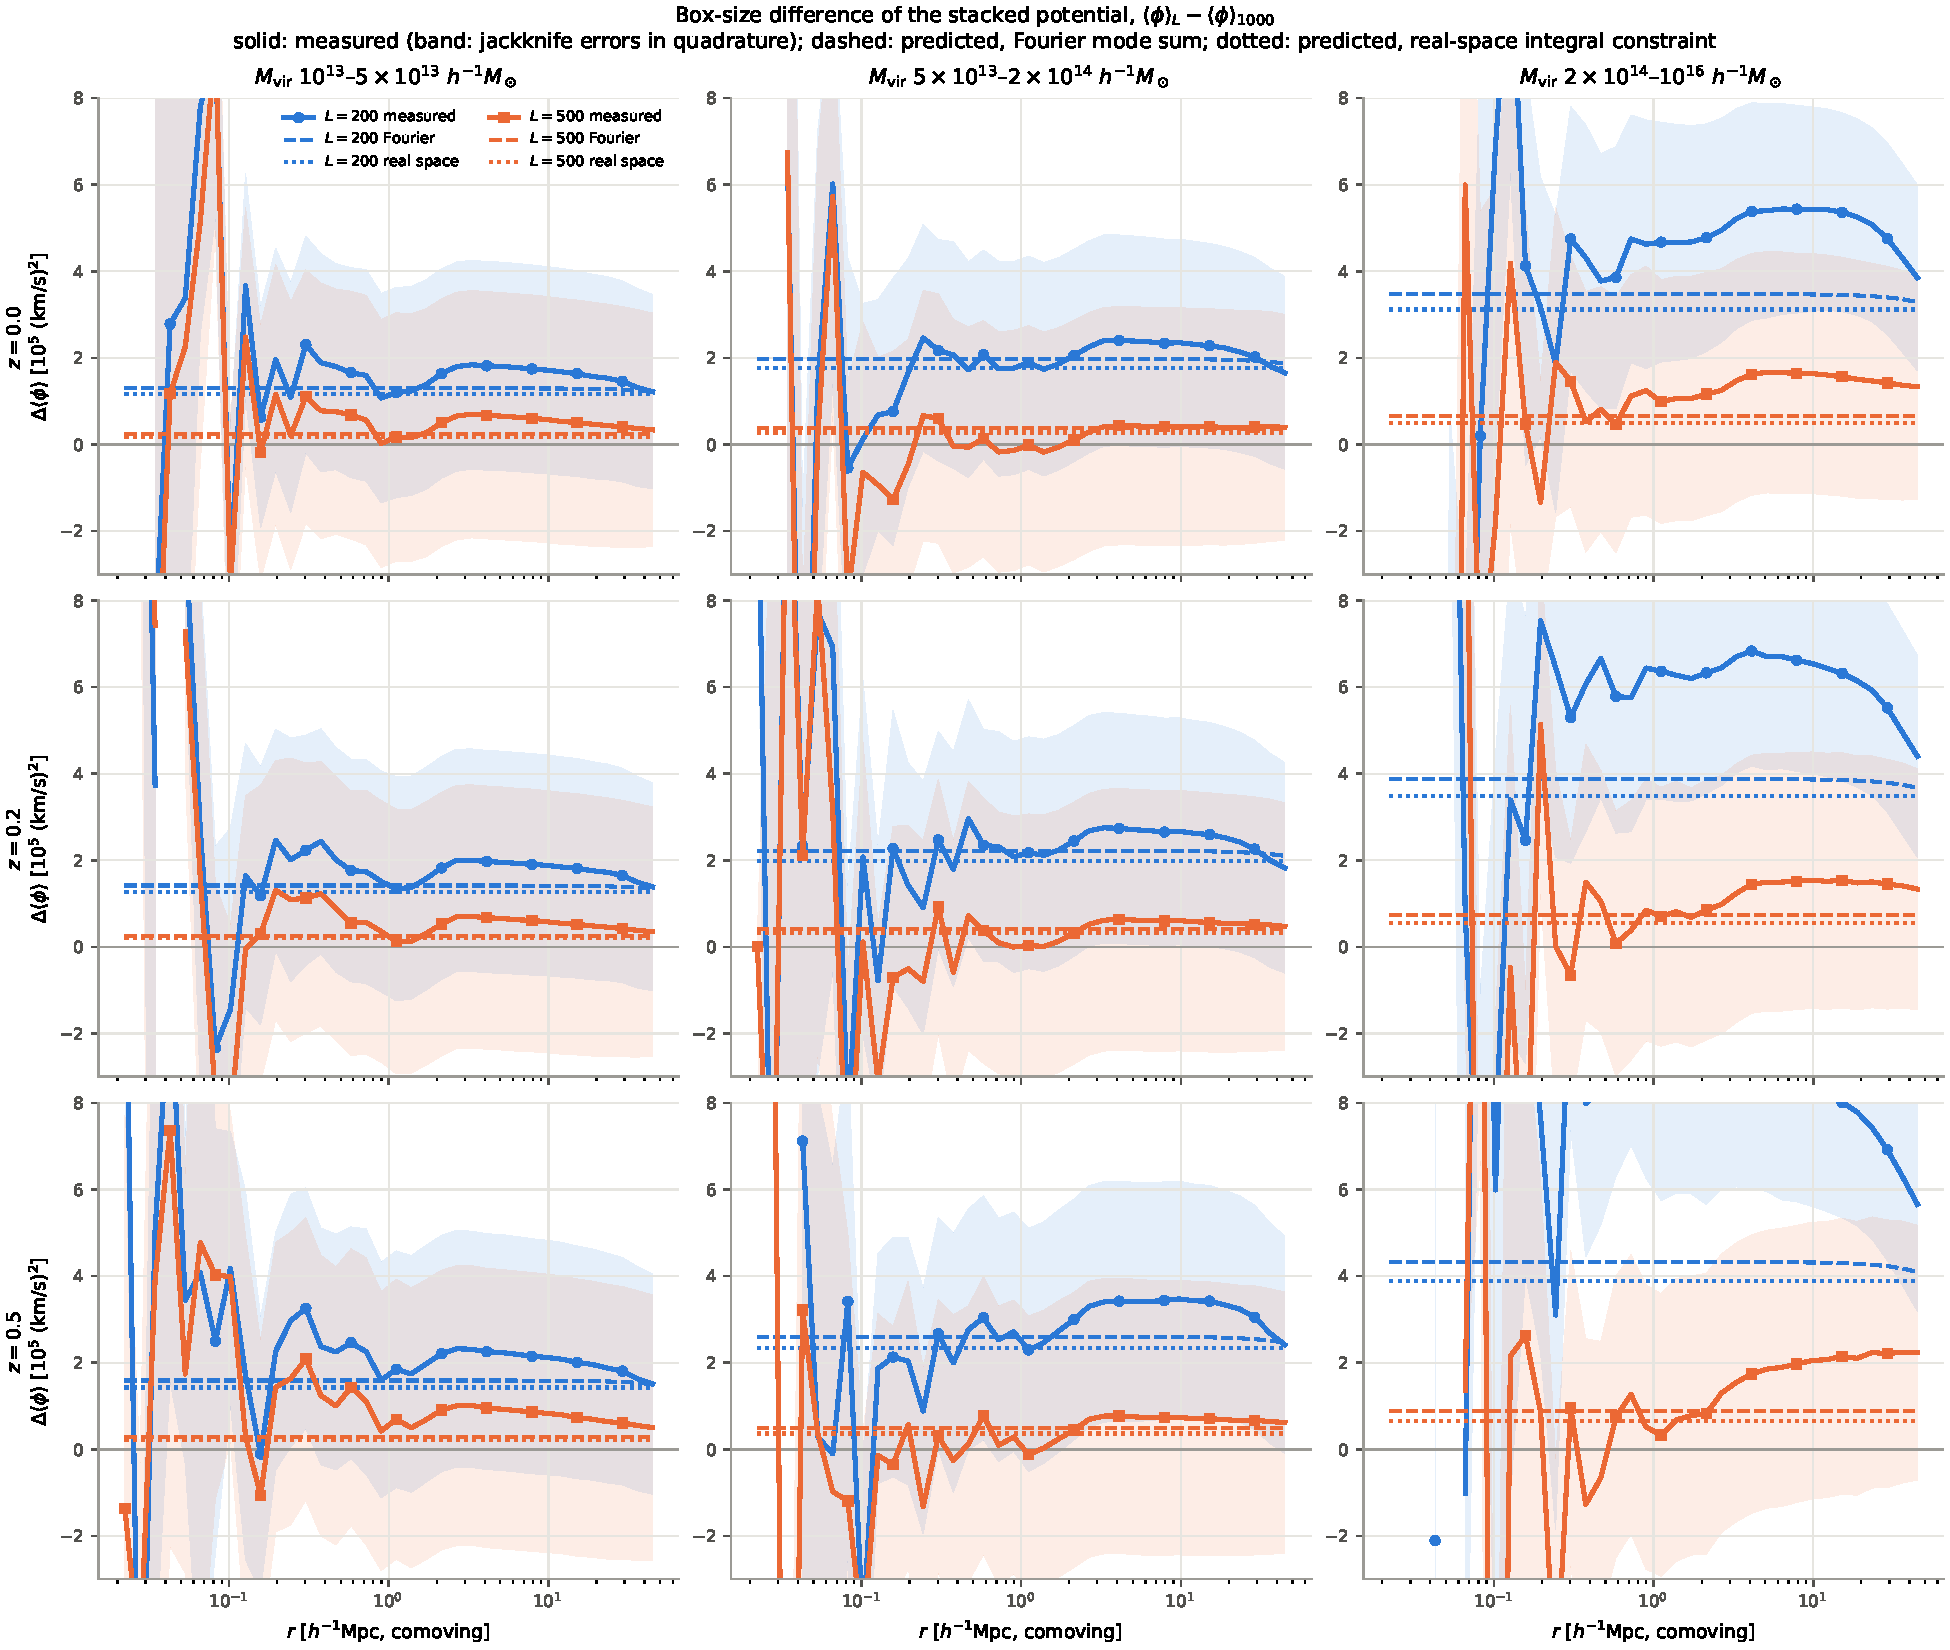
\includegraphics[width=\textwidth]{figs/boxsize_vprof_dphi.pdf}
\caption{Box-size difference of the stacked potential, $\langle\phi\rangle_L-\langle\phi\rangle_{1000}$, for L200
and L500. Solid: measured (band: the two jackknife errors in quadrature). Dashed: predicted difference of the shifts,
Fourier mode sum. Dotted: real-space integral-constraint estimate.}
\label{fig:boxsize_dphi}
\end{figure}

\begin{figure}[H]
\centering
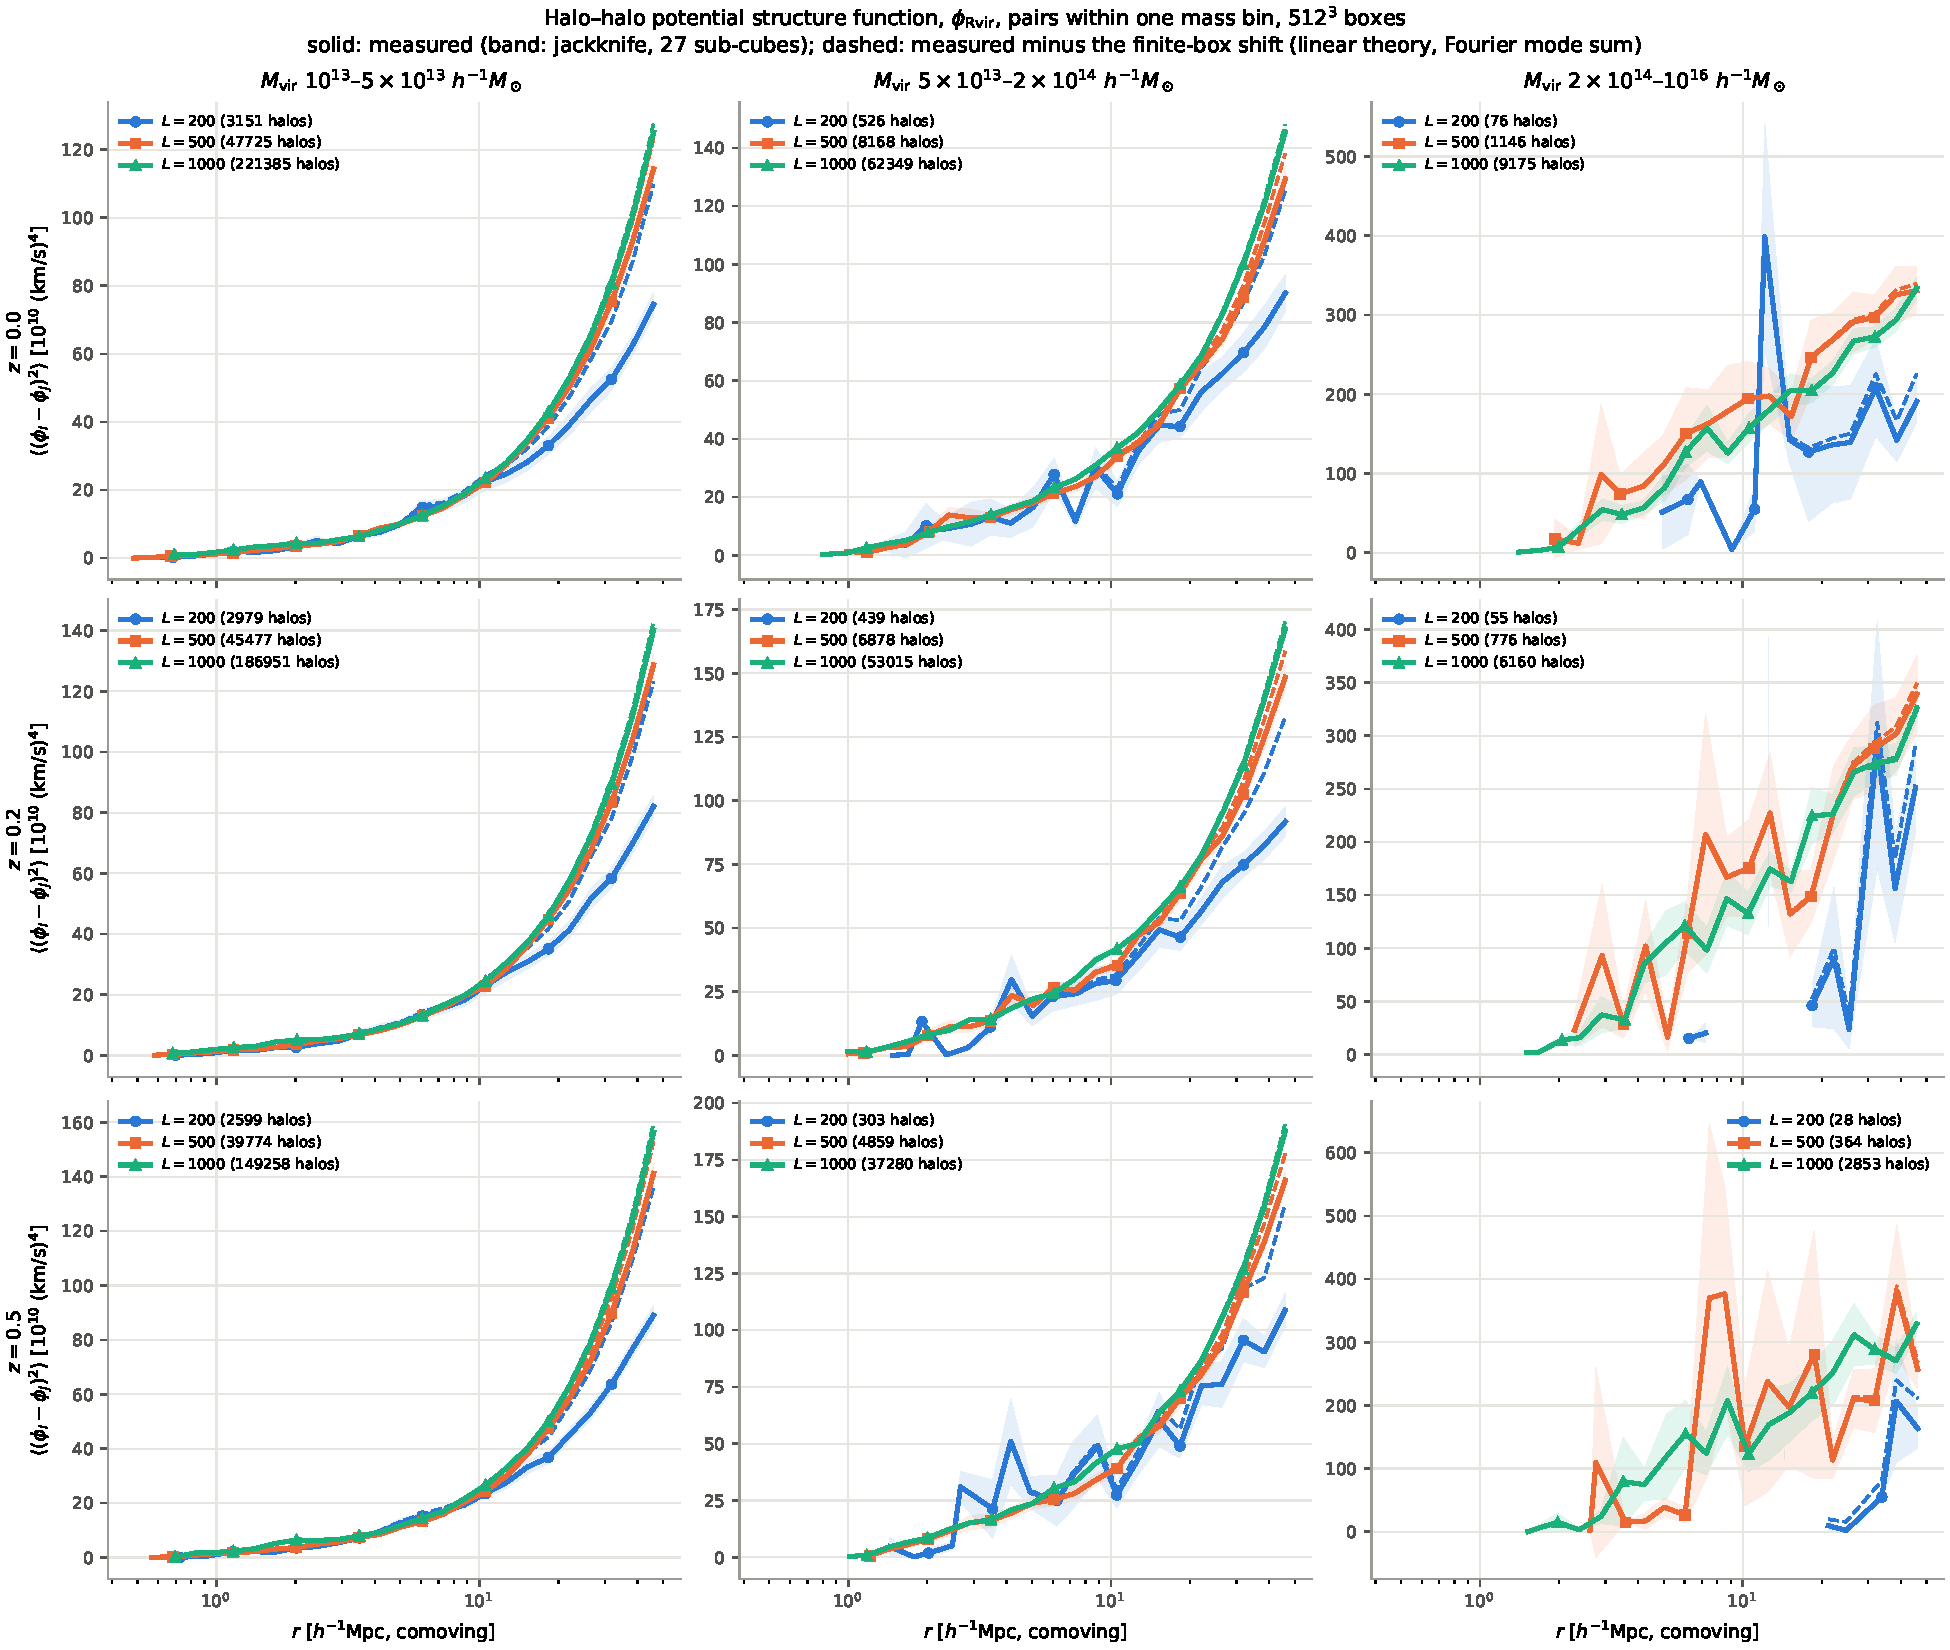
\includegraphics[width=\textwidth]{figs/boxsize_xcorr.pdf}
\caption{Structure function of the halo potentials $\phi_{R_{\rm vir}}$ for pairs within one mass bin, measured
(solid) and corrected by the mode-sum prediction (dashed).}
\label{fig:boxsize_xcorr}
\end{figure}

\begin{figure}[H]
\centering
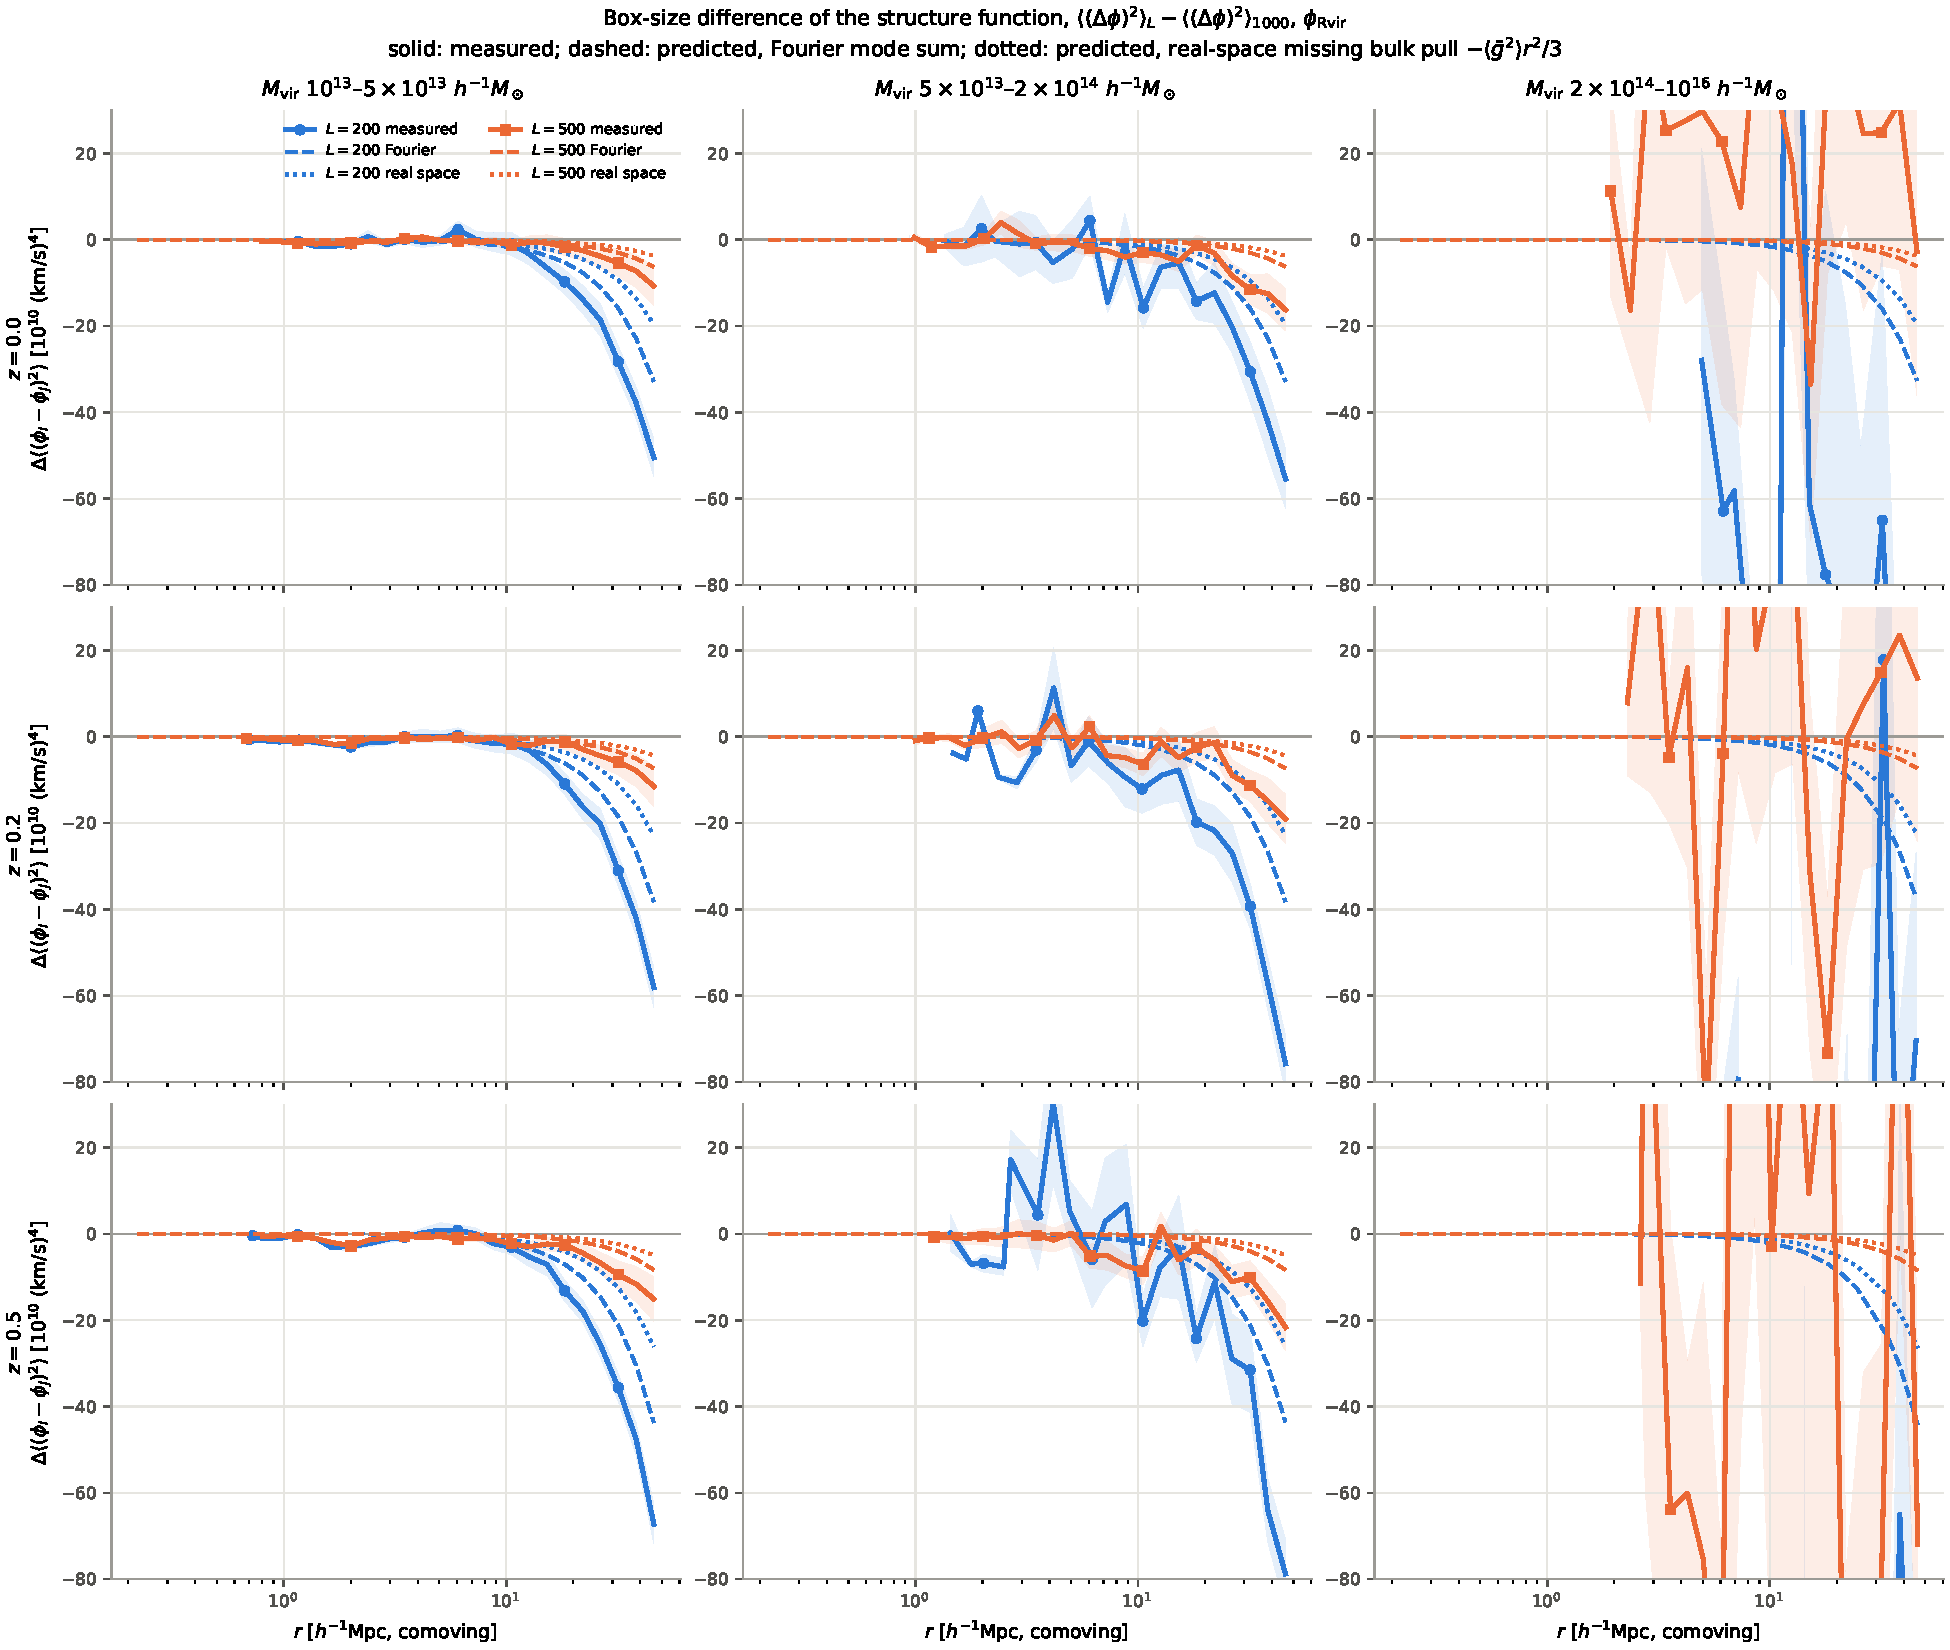
\includegraphics[width=\textwidth]{figs/boxsize_xcorr_dsf.pdf}
\caption{Box-size difference of the structure function relative to L1000. Solid: measured. Dashed: mode sum. Dotted:
real-space missing bulk pull, $-(\langle\bar g^2\rangle_L-\langle\bar g^2\rangle_{1000})\,r^2/3$.}
\label{fig:boxsize_dsf}
\end{figure}

\begin{table}[H]
\centering\footnotesize
% written by make_boxsize_figures.py
\begin{tabular}{cccc cc ccc c}
\toprule
 & & & & \multicolumn{2}{c}{shift of $\langle\phi\rangle$} & \multicolumn{3}{c}{$\langle\phi\rangle_L-\langle\phi\rangle_{1000}$, 1--20\,\Mpch} & missing \\
$z$ & bin & $L$ & $b$ & Fourier & real sp. & measured & Fourier & real sp. & $v_{\rm bulk}$ \\
\midrule
0.0 & 1 & 200 & 1.30 & 1.40 & 1.23 & 1.64 & 1.30 & 1.17 & 194 \\
0.0 & 1 & 500 & 1.30 & 0.34 & 0.25 & 0.51 & 0.24 & 0.18 & 97 \\
0.0 & 1 & 1000 & 1.36 & 0.10 & 0.07 & -- & -- & -- & 52 \\
0.0 & 2 & 200 & 1.97 & 2.12 & 1.87 & 2.22 & 1.97 & 1.77 & 194 \\
0.0 & 2 & 500 & 1.97 & 0.52 & 0.38 & 0.28 & 0.37 & 0.28 & 97 \\
0.0 & 2 & 1000 & 1.98 & 0.15 & 0.10 & -- & -- & -- & 52 \\
0.0 & 3 & 200 & 3.46 & 3.72 & 3.29 & 5.25 & 3.47 & 3.12 & 194 \\
0.0 & 3 & 500 & 3.48 & 0.92 & 0.66 & 1.43 & 0.66 & 0.49 & 97 \\
0.0 & 3 & 1000 & 3.44 & 0.26 & 0.17 & -- & -- & -- & 52 \\
\midrule
0.2 & 1 & 200 & 1.46 & 1.53 & 1.35 & 1.80 & 1.42 & 1.27 & 195 \\
0.2 & 1 & 500 & 1.46 & 0.37 & 0.27 & 0.51 & 0.26 & 0.20 & 97 \\
0.2 & 1 & 1000 & 1.56 & 0.11 & 0.08 & -- & -- & -- & 52 \\
0.2 & 2 & 200 & 2.28 & 2.38 & 2.10 & 2.55 & 2.21 & 1.99 & 195 \\
0.2 & 2 & 500 & 2.29 & 0.58 & 0.42 & 0.46 & 0.42 & 0.31 & 97 \\
0.2 & 2 & 1000 & 2.30 & 0.17 & 0.11 & -- & -- & -- & 52 \\
0.2 & 3 & 200 & 3.98 & 4.16 & 3.67 & 6.46 & 3.87 & 3.48 & 195 \\
0.2 & 3 & 500 & 4.04 & 1.03 & 0.75 & 1.24 & 0.74 & 0.55 & 97 \\
0.2 & 3 & 1000 & 4.00 & 0.29 & 0.19 & -- & -- & -- & 52 \\
\midrule
0.5 & 1 & 200 & 1.79 & 1.71 & 1.51 & 2.10 & 1.59 & 1.43 & 189 \\
0.5 & 1 & 500 & 1.79 & 0.42 & 0.30 & 0.82 & 0.29 & 0.22 & 94 \\
0.5 & 1 & 1000 & 1.93 & 0.13 & 0.09 & -- & -- & -- & 51 \\
0.5 & 2 & 200 & 2.92 & 2.79 & 2.46 & 3.22 & 2.60 & 2.33 & 189 \\
0.5 & 2 & 500 & 2.92 & 0.68 & 0.49 & 0.56 & 0.49 & 0.36 & 94 \\
0.5 & 2 & 1000 & 2.93 & 0.19 & 0.13 & -- & -- & -- & 51 \\
0.5 & 3 & 200 & 4.87 & 4.66 & 4.11 & 8.43 & 4.32 & 3.88 & 189 \\
0.5 & 3 & 500 & 5.24 & 1.22 & 0.89 & 1.53 & 0.89 & 0.66 & 94 \\
0.5 & 3 & 1000 & 5.12 & 0.34 & 0.23 & -- & -- & -- & 51 \\
\bottomrule
\end{tabular}

\caption{Finite-box shift of the stacked potential, in $10^5$\,\kms. Columns 5--6: predicted shift of each box
(mode sum, mean over 1--20\,\Mpch; real-space integral-constraint estimate), with the Tinker bias $b$ of column 4.
Columns 7--9: $\langle\phi\rangle_L-\langle\phi\rangle_{1000}$ averaged over 1--20\,\Mpch{} (inverse-variance
weights), measured and predicted. Last column: 3D rms bulk velocity (km\,s$^{-1}$) of a sphere of the box volume in an
infinite universe, which the periodic box sets to zero.}
\label{tab:boxsize}
\end{table}

\paragraph{Mean potential.} The smaller box is shallower at every radius by an amount that hardly depends on $r$, as
predicted. From 1 to 20\,\Mpch{} at $z = 0$, L200 $-$ L1000 is 1.64, 2.22 and 5.25 in $10^5$\,\kms{} for the three
bins, against 1.30, 1.97 and 3.47 predicted (mode sum; 1.17, 1.77, 3.12 in real space). The first two bins agree to
10--25\%; the top bin of L200 holds 76 halos. L500 $-$ L1000 is 0.51, 0.28 and 1.43 against 0.24, 0.37 and 0.66. The
same pattern holds at $z = 0.2$ and 0.5. Subtracting the predicted shift (Fig.~\ref{fig:boxsize_vprof}, dashed)
brings the three boxes together within the jackknife errors from 0.3 to 50\,\Mpch. The shift is 1.5--3.7, 0.3--0.9
and 0.1--0.26 in $10^5$\,\kms{} for L200, L500, L1000 (bins 1--3, $z = 0$), that is 15--30\%, 4--8\% and 1--2\% of
$\langle\phi\rangle$ at 1\,\Mpch. The jackknife errors (bands) are dominated by the sub-cube-to-sub-cube offsets of the
potential itself and are large compared with the scatter between neighbouring radii.

\paragraph{Structure function.} The boxes agree below $\sim$10\,\Mpch; beyond, the smaller box falls short, growing
as $\sim r^2$. At 38\,\Mpch{} and $z = 0$, L200 $-$ L1000 is $-38$ and $-42$ ($10^{10}$\,(km\,s$^{-1}$)$^4$, bins 1
and 2; L1000 itself is 100 and 121), against $-23$ predicted by the mode sum and $-14$ by the real-space bulk pull;
at $z = 0.5$, $-48$ and $-64$ against $-30$. The prediction has the right shape and redshift dependence but explains
only 50--60\% of the measured deficit, and the measured deficit grows with halo mass while the linear prediction for
the matter potential does not. The missing part is presumably the correlation between where halos sit and the
large-scale potential (halos sample the potential at biased positions), which the unbiased $\xi_{\phi\phi}$ ignores;
differences in mass resolution between the boxes may contribute as well. The top bin is too sparse in L200 to say
anything.

\paragraph{Consequences.} At $200$\,\Mpch, the box shifts the mean potential around halos by $\sim(1.5$--$4)\times
10^5$\,\kms{} at all radii, about ten times the code-to-code differences of the stacked potential in the earlier sections, and lowers the
halo--halo potential structure function at $r\gtrsim10$\,\Mpch{} by up to $\sim40\%$ at 40\,\Mpch. Both should be
corrected (or the box size stated) when comparing with larger volumes or with theory; for the mean potential the
linear correction above is adequate at the 10--25\% level, for the structure function it is not yet.
